\documentclass[12pt]{beamer}
\newenvironment{ConCodigo}[1]
  {\begin{frame}[fragile,environment=ConCodigo]{#1}}
  {\end{frame}}
\graphicspath{{Imagenes/}{../Imagenes/}}
\usepackage[utf8]{inputenc}
\usepackage[spanish]{babel}
\usepackage{hyperref}
\usepackage{etex}
%\reserveinserts{28}
\usepackage{amsmath}
\usepackage{amsthm}
\usepackage{mathtools}
\usepackage{multicol}
\usepackage{multirow}
\usepackage{tabulary}
\usepackage{booktabs}
\usepackage{nccmath}
\usepackage{physics}
\usepackage{biblatex}
\usepackage[outdir=./]{epstopdf}
%\epstopdfsetup{outdir=./}
\usepackage{graphicx}
%\usepackage{enumitem,xcolor}
\usepackage{siunitx}
%\sisetup{scientific-notation=true}
%\usepackage{fontspec}
\usepackage{lmodern}
\usepackage{float}
\usepackage[format=hang, font=footnotesize, labelformat=parens]{caption}
\usepackage[autostyle,spanish=mexican]{csquotes}
\usepackage{standalone}
\usepackage{blkarray}
\usepackage{algorithm}
\usepackage{algorithmic}
\usepackage{tikz}
\usepackage[siunitx, RPvoltages]{circuitikz}
\usetikzlibrary{arrows,patterns,shapes}
\usetikzlibrary{decorations.markings}
\usetikzlibrary{arrows}
\usepackage{color}
\usepackage{xcolor}
%\usepackage{beton}
%\usepackage{euler}
%\usepackage[T1]{fontenc}
\usepackage[sfdefault]{roboto}  %% Option 'sfdefault' only if the base font of the document is to be sans serif
\usepackage[T1]{fontenc}
\renewcommand*\familydefault{\sfdefault}
\DeclareGraphicsExtensions{.pdf,.png,.jpg}
\usepackage{hyperref}
\renewcommand {\arraystretch}{1.5}
\newcommand{\python}{\texttt{python}}
\usefonttheme[onlymath]{serif}
\setbeamertemplate{navigation symbols}{}
\usetikzlibrary{patterns}
\usetikzlibrary{decorations.markings}
\tikzstyle{every picture}+=[remember picture,baseline]
%\tikzstyle{every node}+=[inner sep=0pt,anchor=base,
%minimum width=2.2cm,align=center,text depth=.15ex,outer sep=1.5pt]
%\tikzstyle{every path}+=[thick, rounded corners]
\setbeamertemplate{caption}[numbered]
\newcommand{\ptm}{\fontfamily{ptm}\selectfont}
%Se usa la plantilla Warsaw modificada con spruce
\mode<presentation>
{
  \usetheme{Warsaw}
  \setbeamertemplate{headline}{}
  \useoutertheme{default}
  \usecolortheme{albatross}
  \setbeamercovered{invisible}
}
% \AtBeginSection[]
% {
% \begin{frame}<beamer>{Contenido}
% \normalfont\mdseries
% \tableofcontents[currentsection]
% \end{frame}
% }

\include{pre_codigo}
\begin{document}
\title{Examen 1 - Errores, Condición y Estabilidad}
\subtitle{C\'alculo de ra\'{i}ces - Soluci\'{o}n}
%\subsubtitle{Curso de F\'{i}sica Computacional}
\author{M. en C. Gustavo Contreras Mayén}
%\email{curso.fisica.comp@gmail.com}
%\ptsize{10}
\maketitle
\fontsize{14}{14}\selectfont
\spanishdecimal{.}
\begin{frame}{Contenido}
\tableofcontents[pausesections]
\end{frame}
\section{Problema 1}
\begin{frame}
\frametitle{Problema 1}
Calcula el error absoluto y el error relativo en las aproximaciones de $p$ y $p^{*}$:
\begin{multicols}{2}
\begin{enumerate}
\item $p = \pi$, $p^{*} = 22/7$
\item $p = \pi$, $p^{*} = 3.1416$
\item $p = e$, $p^{*} = 2.718$
\item $e = \sqrt{2}$, $p^{*} = 1.414$
\item $p= e^{10}$, $p^{*} = 22000$
\item $p= 10^{\pi}$, $p^{*} = 1400$
\item $p = 8!$, $p^{*}=39900$
\item $p = 9!$, $p^{*}= \sqrt{18 \pi} (9/e)^{9}$
\end{enumerate}
\end{multicols}
\end{frame}
\begin{frame}
\frametitle{Solución}
\begin{tabular}{l | c | c}
\hline
Inciso & Error absoluto & Error relativo \\ \hline
a) & $1.234489e-03$ & $4.02499e-04$ \\ \hline
b) & $7.346410e-06$ & $2.338435e-06$ \\ \hline
c) & $2.818285e-04$ & $1.036789e-04$ \\ \hline
d) & $2.135624e-04$ & $1.510114e-04$ \\ \hline
e) & $1.454427e+01$ & $1.049782e-02$ \\ \hline
f) & $420$ & $1.052632e-02$ \\ \hline
g) & $3.343127e+03$ & $9.2212762e-03$ \\ \hline
\end{tabular}
\end{frame}
\begin{frame}
\frametitle{Problema 2}
Calcula $\frac{122}{135} - \frac{11}{32} + \frac{20}{19}$ mediante aritmética exacta, utiliza truncamiento a tres cifras y redondeo hasta tres cifras. Determina los errores absolutos y relativos.
\pause
\\
\medskip
Solución:
\\
\medskip
Haciendo primeramente el quebrado, tenemos que:
\[ \dfrac{122}{135} - \dfrac{11}{32} + \dfrac{20}{19} = \dfrac{132361}{82080} = 1.6125852826 \]
\begin{tabular}{l | c | c}
\hline
Operación & Error absoluto & Error relativo \\ \hline
Red. ($1.613$) & $4.147173e-04$ & $2.571755e-04$ \\ \hline
Trunc. ($1.612$) & $5.852827e-04$ & $3.629468e-04$ \\ \hline
\end{tabular}
\end{frame}
\begin{frame}
\frametitle{Problema 3}
Las expresiones $215 -0.345-214$ y $215-214-0.345$ son idénticas. Calcula mediante aritmética exacta el resultado, luego usa truncamiento y redondeo hasta tres cifras. Determina los errores absoluto y relativo. 
\pause
El valor exacto es: $0.655$, por lo que
\begin{tabular}{l | c | c}
\hline
Operación & Error absoluto & Error relativo \\ \hline
Red. ($0.656$) & $1.110223e-15$ & $1.694997e-15$ \\ \hline
Trunc. ($0.655$) & $0$ & $0$ \\ \hline
\end{tabular}
\end{frame}
\begin{frame}
\frametitle{Problema 4}
Se sabe que
\[ \pi = 4 - 8 \sum_{k=1}^{\infty} \left( 16 k^{2} - 1 \right)^{-1} \]
¿Cuántas iteraciones se necesitan para producir el resultado con diez cifras decimales de exactitud?
\end{frame}
\begin{frame}[fragile]
\frametitle{Problema 5}
Compara gráficamente el valor entre la función y las primeras cinco sumas parciales de la serie
\[ \arctan(x) = \sum_{k=1}^{\infty} (-1)^{k+1} \dfrac{x^{2k-1}}{2k-1}\]
\end{frame}
\begin{frame}
\frametitle{Gráfica con la función y términos de la serie}
\begin{figure}
	\centering
	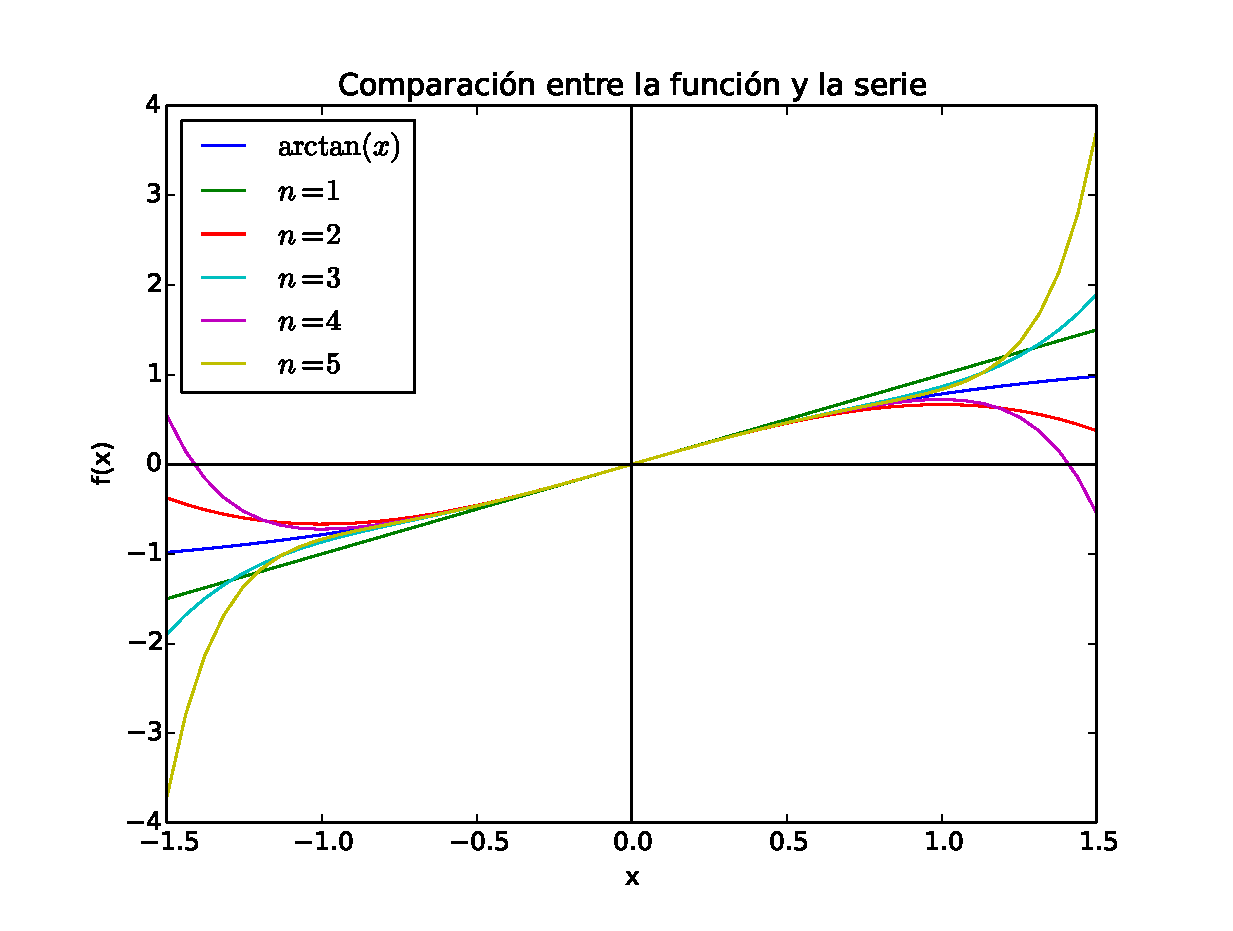
\includegraphics[scale=0.5]{Imagenes/Problema_5_2015_1.eps} 
\end{figure}
\end{frame}
\begin{frame}
\frametitle{Problema 6}
Usando la serie de Maclaurin truncada, una función $f(x)$ con $n$ derivadas continuas se puede aproximar con un polinomio de n-ésimo grado
\[ f(x) \simeq p_{n}(x) = \sum_{i=0}^{n} c_{i} x^{i} \]
donde $c_{i} = \dfrac{f^{(i)}(0)}{i!}$
Genera y compara las gráficas para $f(x)= e^{x}$ y los polinomios $p_{2}(x)$, $p_{3}(x)$, $p_{4}(x)$, $p_{5}(x)$. Discute tus resultados.
\end{frame}
\begin{frame}[fragile]
\frametitle{Gráfica con la función y términos de la serie}
\begin{figure}
	\centering
	\includegraphics[scale=0.5]{Imagenes/Problema_6_2015_1.eps} 
\end{figure}
\end{frame}
\begin{frame}
\frametitle{Problema 9}
Las siguientes expresiones definen a la constante de Euler
\begin{eqnarray}
\gamma &=& \lim_{n \rightarrow \infty} \left[ \sum_{k=1}^{n} \dfrac{1}{k} - ln (n) \right] \\
\gamma &=& \lim_{k \rightarrow \infty} \left[ \sum_{k=1}^{m} \dfrac{1}{k} - ln \left( m + \dfrac{1}{2} \right) \right]
\end{eqnarray}
Escribe un programa que calcule el valor de $\gamma = 0.57721$, ¿cuál de las dos expresiones converge más rápido al valor?
\end{frame}
\end{document}